% ****** Start of file aipsamp.tex ******
%
%   This file is part of the AIP files in the AIP distribution for REVTeX 4.
%   Version 4.1 of REVTeX, October 2009
%
%   Copyright (c) 2009 American Institute of Physics.

% Use this file as a source of example code for your aip document.
% Use the file aiptemplate.tex as a template for your document.
\documentclass[%
 aip,
 jmp,%
 amsmath,amssymb,
%preprint,%
 reprint,%
 floatfix,
%author-year,%
%author-numerical,%
]{revtex4-1}
\usepackage{graphicx}% Include figure files
\usepackage{grffile}
\usepackage{dcolumn}% Align table columns on decimal point
\usepackage{bm}% bold math
%\usepackage[mathlines]{lineno}% Enable numbering of text and display math
%\linenumbers\relax % Commence numbering lines
\usepackage{multirow}
\usepackage{color} % for the notes
\usepackage{etex}
\reserveinserts{58}
%\usepackage{morefloats}
\usepackage{hyperref}
\usepackage{xcolor}
\usepackage{amsmath}
\hypersetup{
        colorlinks,
        linkcolor={red!50!black},
        citecolor={blue!50!black},
        urlcolor={blue!80!black}
}
%\usepackage{placeins}
\usepackage{xr}
\externaldocument{paper}
\usepackage[section] {placeins}

\begin{document}

\preprint{XXXXX (preprint)}

%\title[Evolution of interaction networks]{On the evolution of interaction networks: primitive typology of vertex, prominence of measures and activity statistics}% Force line breaks with \\
%\title[Evolution of interaction networks]{On the evolution of interaction networks: a primitive typology of vertex}% Force line breaks with \\
\title[Stability of interaction networks, SUPPORTING INFORMATION]{Stability in human interaction networks: primitive typology of vertex, prominence of measures and time activity statistics, SUPPORTING INFORMATION}% Force line breaks with \\

\author{Renato Fabbri}%
 \homepage{http://ifsc.usp.br/~fabbri/}
 \email{fabbri@usp.br}
  \affiliation{ 
S\~ao Carlos Institute of Physics, University of S\~ao Paulo (IFSC/USP)%\\This line break forced with \textbackslash\textbackslash
}

\author{Vilson V. da Silva Jr.}
  \homepage{http://automata.cc/}
  \email{vilson@void.cc}
  \altaffiliation[Also at ]{IFSC-USP}%Lines break automatically or can be forced with \\

\author{Ricardo Fabbri}
  \homepage{http://www.lems.brown.edu/~rfabbri/}
  \email{rfabbri@iprj.uerj.br}
 \altaffiliation{
Instituto Polit\'ecnico, Universidade Estadual do Rio de Janeiro (IPRJ)
}%Lines break automatically or can be forced with \\

\author{Deborah C. Antunes}
  \homepage{http://lattes.cnpq.br/1065956470701739}
  \email{deborahantunes@gmail.com}
  \altaffiliation{
Curso de Psicologia, Universidade Federal do Cer\'a (UFC)
}%Lines break automatically or can be forced with \\

\author{Marilia M. Pisani}
  \homepage{http://lattes.cnpq.br/6738980149860322}
  \email{marilia.m.pisani@gmail.com}
 \altaffiliation{
Centro de Ciências Naturais e Humanas, Universidade Federal do ABC (CCNH/UFABC)
}%Lines break automatically or can be forced with \\

%
%%\author{Luciano da Fontoura Costa}
%%  \homepage{http://cyvision.ifsc.usp.br/~luciano/}
%%  \email{ldfcosta@gmail.com}
%  \altaffiliation[Also at ]{IFSC-USP}%Lines break automatically or can be forced with \\

%\author{Osvaldo N. Oliveira Jr.}
%  \homepage{www.polimeros.ifsc.usp.br/professors/professor.php?id=4}
%  \email{chu@ifsc.usp.br}
% \altaffiliation[Also at ]{IFSC-USP}%Lines break automatically or can be forced with \\


\date{\today}% It is always \today, today,
             %  but any date may be explicitly specified

\begin{abstract}
 This is the supporting information of the article that reports interaction networks stability by means of three quantitative criteria: activity distribution in time and among participants; a sound classification of vertices in peripheral, intermediary and hub sectors; the combination of basic measures into principal components with greater variance. 
\end{abstract}

\pacs{89.75.Fb,05.65.+b,89.65.-s}% PACS, the Physics and Astronomy
\keywords{complex networks, social network analysis, pattern recognition, statistics, anthropological physics}
\maketitle

These results were produced with the Gmane public domain data and an open python package designed for attaining
these, and related, results. The interested reader should follow Appendix~\ref{scripts} to access both data and rotines.
Inline are results for 4 emails lists: LAD, LAU, MET and CPP, as described in Section~\ref{sec:data}.
Similar results can be reproduced for any number of (Gmane) email lists.
To avoid repeating text of each table for each list, the text is given inline.

\section{Time tables in different scales}\label{sec:time}
Theory presented in Section~\ref{sec:mtime} and results exposed in Section~\ref{constDisc} of the paper~\cite{tpaper}.
\subsection{Time circular measures}
The rescaled circular mean $\theta_\mu'$, the standard deviation $S(z)$, the variance $Var(z)$, the circular dispersion $\delta(z)$ and the relation of maximum and minimum incidence at each time unit $\frac{max(incidence}{min(incidence}$. Also, $ \mu_{\frac{max(incidence')}{min(incidence')}} $ and $ \sigma_{\frac{max(incidence')}{min(incidence')} }$ are given for 1000 uniform distribution simulations within the same number of bins and with the same number of samples. Section~\ref{sec:mtime} describes the theoretical background of directional (or circular) statistics.
\begin{table*}[!h]
	\caption{LAU circular measures}
\begin{center}
    \begin{tabular}{ |l|| c|c|c|c|c||c|c| }
        \hline
scale & $\theta_\mu'$ & $S(z)$ & $Var(z)$ & $\delta(z)$ & $\frac{max(incidence)}{min(incidence)}$ & $ \mu_{\frac{max(incidence')}{min(incidence')}} $ & $ \sigma_{\frac{max(incidence')}{min(incidence')} } $ \\ \hline\hline
	seconds & --//--  & 3.31  & 1.00  & 29337.65  & 1.27  & 1.29  & 0.04 \\\hline
minutes & --//--  & 3.13  & 0.99  & 8879.19  & 1.32  & 1.29  & 0.04 \\\hline
hours & -8.76  & 1.56  & 0.71  & 4.92  & 8.38  & 1.14  & 0.03 \\\hline
weekdays & -0.21  & 2.14  & 0.90  & 45.41  & 1.62  & 1.05  & 0.02 \\\hline
month days & -0.64  & 2.76  & 0.98  & 1001.75  & 1.49  & 1.17  & 0.03 \\\hline
months & 3.55  & 2.30  & 0.93  & 94.53  & 1.57  & 1.09  & 0.02 \\\hline

    \end{tabular}
\end{center}
\label{tab:circ}
\end{table*}
\begin{table*}[!h]
	\caption{LAD circular measures}
\begin{center}
    \begin{tabular}{ |l|| c|c|c|c|c||c|c| }
        \hline
scale & $\theta_\mu'$ & $S(z)$ & $Var(z)$ & $\delta(z)$ & $\frac{max(incidence)}{min(incidence)}$ & $ \mu_{\frac{max(incidence')}{min(incidence')}} $ & $ \sigma_{\frac{max(incidence')}{min(incidence')} } $ \\ \hline\hline
	seconds & --//--  & 3.13  & 0.99  & 9070.17  & 1.28  & 1.29  & 0.05 \\\hline
minutes & --//--  & 3.60  & 1.00  & 205489.40  & 1.22  & 1.29  & 0.05 \\\hline
hours & -9.61  & 1.52  & 0.68  & 4.36  & 9.77  & 1.15  & 0.03 \\\hline
weekdays & -0.03  & 2.03  & 0.87  & 29.28  & 1.72  & 1.05  & 0.02 \\\hline
month days & -0.07  & 2.94  & 0.99  & 2754.16  & 2.21  & 1.17  & 0.03 \\\hline
months & -0.56  & 2.14  & 0.90  & 44.00  & 2.25  & 1.09  & 0.02 \\\hline

    \end{tabular}
\end{center}
\label{tab:circ}
\end{table*}
\begin{table*}[!h]
	\caption{MET circular measures}
\begin{center}
    \begin{tabular}{ |l|| c|c|c|c|c||c|c| }
        \hline
scale & $\theta_\mu'$ & $S(z)$ & $Var(z)$ & $\delta(z)$ & $\frac{max(incidence)}{min(incidence)}$ & $ \mu_{\frac{max(incidence')}{min(incidence')}} $ & $ \sigma_{\frac{max(incidence')}{min(incidence')} } $ \\ \hline\hline
	seconds & --//--  & 3.06  & 0.99  & 5910.47  & 1.27  & 1.29  & 0.04 \\\hline
minutes & --//--  & 3.14  & 0.99  & 9696.29  & 1.34  & 1.29  & 0.04 \\\hline
hours & -9.20  & 1.35  & 0.60  & 2.76  & 19.26  & 1.14  & 0.03 \\\hline
weekdays & -0.27  & 1.86  & 0.82  & 13.82  & 2.89  & 1.05  & 0.02 \\\hline
month days & 3.58  & 2.49  & 0.95  & 237.30  & 1.55  & 1.17  & 0.03 \\\hline
months & -2.92  & 1.73  & 0.78  & 9.20  & 3.04  & 1.09  & 0.02 \\\hline

    \end{tabular}
\end{center}
\label{tab:circ}
\end{table*}
\begin{table*}[!h]
	\caption{CPP circular measures}
\begin{center}
    \begin{tabular}{ |l|| c|c|c|c|c||c|c| }
        \hline
scale & $\theta_\mu'$ & $S(z)$ & $Var(z)$ & $\delta(z)$ & $\frac{max(incidence)}{min(incidence)}$ & $ \mu_{\frac{max(incidence')}{min(incidence')}} $ & $ \sigma_{\frac{max(incidence')}{min(incidence')} } $ \\ \hline\hline
	seconds & --//--  & 3.31  & 1.00  & 28205.46  & 0.79  & 0.78  & 0.03 \\\hline
minutes & --//--  & 3.18  & 0.99  & 12275.59  & 0.79  & 0.78  & 0.03 \\\hline
hours & -9.39  & 1.48  & 0.67  & 3.91  & 0.09  & 0.87  & 0.02 \\\hline
weekdays & -0.17  & 1.83  & 0.81  & 12.66  & 0.39  & 0.95  & 0.01 \\\hline
month days & -10.12  & 3.16  & 0.99  & 10789.17  & 0.65  & 0.85  & 0.02 \\\hline
months & 0.15  & 2.34  & 0.93  & 115.49  & 0.67  & 0.92  & 0.02 \\\hline

    \end{tabular}
\end{center}
\label{tab:circ}
\end{table*}

\FloatBarrier
\subsection{Time histograms}
\subsection{Histograms of activity along the hours of the day}

Activity percentages along the hours of the day. Higher activity was observed between noon and 6pm, followed by the time period between 6pm and midnight. Around 2/3 of the whole activity takes place from noon to midnight. Nevertheless, the activity peak occurs around midday, with a slight skew toward one hour before noon.
\begin{table}[!h]
	\caption{LAU activity along the hours of the day}
	\footnotesize
	\begin{center}
\begin{tabular}{l || c | c | c | c | c | c |}\hline
 & 1h & 2h & 3h & 4h & 6h & 12h \\\hline
0h & \multirow{1}{*}{ 3.58 }  & \multirow{2}{*}{ 5.80 }  & \multirow{3}{*}{ 7.43 }  & \multirow{4}{*}{ 8.49 }  & \multirow{6}{*}{ 10.14 }  & \multirow{12}{*}{ 36.88 }  \\\cline{1-1}
1h & \multirow{1}{*}{ 2.22 }  & & & & & \\\cline{1-1}\cline{2-2}
2h & \multirow{1}{*}{ 1.63 }  & \multirow{2}{*}{ 2.69 }  & & & & \\\cline{1-1}\cline{3-3}
3h & \multirow{1}{*}{ 1.06 }  & & \multirow{3}{*}{ 2.72 }  & & & \\\cline{1-1}\cline{2-2}\cline{4-4}
4h & \multirow{1}{*}{ 0.84 }  & \multirow{2}{*}{ 1.66 }  & & \multirow{4}{*}{ 5.20 }  & & \\\cline{1-1}
5h & \multirow{1}{*}{ 0.82 }  & & & & & \\\cline{1-1}\cline{2-2}\cline{3-3}\cline{5-5}
6h & \multirow{1}{*}{ 1.17 }  & \multirow{2}{*}{ 3.54 }  & \multirow{3}{*}{ 7.07 }  & & \multirow{6}{*}{ 26.74 }  & \\\cline{1-1}
7h & \multirow{1}{*}{ 2.37 }  & & & & & \\\cline{1-1}\cline{2-2}\cline{4-4}
8h & \multirow{1}{*}{ 3.53 }  & \multirow{2}{*}{ 9.57 }  & & \multirow{4}{*}{ 23.20 }  & & \\\cline{1-1}\cline{3-3}
9h & \multirow{1}{*}{ 6.04 }  & & \multirow{3}{*}{ 19.67 }  & & & \\\cline{1-1}\cline{2-2}
10h & \multirow{1}{*}{ 6.83 }  & \multirow{2}{*}{ 13.62 }  & & & & \\\cline{1-1}
11h & \multirow{1}{*}{ 6.79 }  & & & & & \\\cline{1-1}\cline{2-2}\cline{3-3}\cline{4-4}\cline{5-5}\cline{6-6}
12h & \multirow{1}{*}{ 6.11 }  & \multirow{2}{*}{ 12.36 }  & \multirow{3}{*}{ 18.75 }  & \multirow{4}{*}{ 24.68 }  & \multirow{6}{*}{ 35.66 }  & \multirow{12}{*}{ 63.12 }  \\\cline{1-1}
13h & \multirow{1}{*}{ 6.26 }  & & & & & \\\cline{1-1}\cline{2-2}
14h & \multirow{1}{*}{ 6.38 }  & \multirow{2}{*}{ 12.31 }  & & & & \\\cline{1-1}\cline{3-3}
15h & \multirow{1}{*}{ 5.93 }  & & \multirow{3}{*}{ 16.91 }  & & & \\\cline{1-1}\cline{2-2}\cline{4-4}
16h & \multirow{1}{*}{ 5.52 }  & \multirow{2}{*}{ 10.98 }  & & \multirow{4}{*}{ 20.73 }  & & \\\cline{1-1}
17h & \multirow{1}{*}{ 5.46 }  & & & & & \\\cline{1-1}\cline{2-2}\cline{3-3}\cline{5-5}
18h & \multirow{1}{*}{ 5.23 }  & \multirow{2}{*}{ 9.75 }  & \multirow{3}{*}{ 14.30 }  & & \multirow{6}{*}{ 27.46 }  & \\\cline{1-1}
19h & \multirow{1}{*}{ 4.52 }  & & & & & \\\cline{1-1}\cline{2-2}\cline{4-4}
20h & \multirow{1}{*}{ 4.55 }  & \multirow{2}{*}{ 8.97 }  & & \multirow{4}{*}{ 17.71 }  & & \\\cline{1-1}\cline{3-3}
21h & \multirow{1}{*}{ 4.42 }  & & \multirow{3}{*}{ 13.16 }  & & & \\\cline{1-1}\cline{2-2}
22h & \multirow{1}{*}{ 4.51 }  & \multirow{2}{*}{ 8.74 }  & & & & \\\cline{1-1}
23h & \multirow{1}{*}{ 4.23 }  & & & & & \\\cline{1-1}\cline{2-2}\cline{3-3}\cline{4-4}\cline{5-5}\cline{6-6}
\end{tabular}
\end{center}
\end{table}

\begin{table}[!h]
	\caption{LAD activity along the hours of the day}
	\footnotesize
	\begin{center}
\begin{tabular}{l || c | c | c | c | c | c |}\hline
 & 1h & 2h & 3h & 4h & 6h & 12h \\\hline
0h & \multirow{1}{*}{ 4.01 }  & \multirow{2}{*}{ 6.53 }  & \multirow{3}{*}{ 8.32 }  & \multirow{4}{*}{ 9.37 }  & \multirow{6}{*}{ 10.78 }  & \multirow{12}{*}{ 33.11 }  \\\cline{1-1}
1h & \multirow{1}{*}{ 2.52 }  & & & & & \\\cline{1-1}\cline{2-2}
2h & \multirow{1}{*}{ 1.79 }  & \multirow{2}{*}{ 2.84 }  & & & & \\\cline{1-1}\cline{3-3}
3h & \multirow{1}{*}{ 1.06 }  & & \multirow{3}{*}{ 2.46 }  & & & \\\cline{1-1}\cline{2-2}\cline{4-4}
4h & \multirow{1}{*}{ 0.75 }  & \multirow{2}{*}{ 1.40 }  & & \multirow{4}{*}{ 3.81 }  & & \\\cline{1-1}
5h & \multirow{1}{*}{ 0.66 }  & & & & & \\\cline{1-1}\cline{2-2}\cline{3-3}\cline{5-5}
6h & \multirow{1}{*}{ 0.85 }  & \multirow{2}{*}{ 2.41 }  & \multirow{3}{*}{ 5.36 }  & & \multirow{6}{*}{ 22.33 }  & \\\cline{1-1}
7h & \multirow{1}{*}{ 1.56 }  & & & & & \\\cline{1-1}\cline{2-2}\cline{4-4}
8h & \multirow{1}{*}{ 2.95 }  & \multirow{2}{*}{ 7.61 }  & & \multirow{4}{*}{ 19.93 }  & & \\\cline{1-1}\cline{3-3}
9h & \multirow{1}{*}{ 4.66 }  & & \multirow{3}{*}{ 16.98 }  & & & \\\cline{1-1}\cline{2-2}
10h & \multirow{1}{*}{ 5.92 }  & \multirow{2}{*}{ 12.32 }  & & & & \\\cline{1-1}
11h & \multirow{1}{*}{ 6.40 }  & & & & & \\\cline{1-1}\cline{2-2}\cline{3-3}\cline{4-4}\cline{5-5}\cline{6-6}
12h & \multirow{1}{*}{ 6.41 }  & \multirow{2}{*}{ 12.53 }  & \multirow{3}{*}{ 18.85 }  & \multirow{4}{*}{ 24.82 }  & \multirow{6}{*}{ 37.24 }  & \multirow{12}{*}{ 66.89 }  \\\cline{1-1}
13h & \multirow{1}{*}{ 6.12 }  & & & & & \\\cline{1-1}\cline{2-2}
14h & \multirow{1}{*}{ 6.32 }  & \multirow{2}{*}{ 12.29 }  & & & & \\\cline{1-1}\cline{3-3}
15h & \multirow{1}{*}{ 5.97 }  & & \multirow{3}{*}{ 18.39 }  & & & \\\cline{1-1}\cline{2-2}\cline{4-4}
16h & \multirow{1}{*}{ 6.40 }  & \multirow{2}{*}{ 12.42 }  & & \multirow{4}{*}{ 23.44 }  & & \\\cline{1-1}
17h & \multirow{1}{*}{ 6.02 }  & & & & & \\\cline{1-1}\cline{2-2}\cline{3-3}\cline{5-5}
18h & \multirow{1}{*}{ 5.99 }  & \multirow{2}{*}{ 11.02 }  & \multirow{3}{*}{ 15.65 }  & & \multirow{6}{*}{ 29.65 }  & \\\cline{1-1}
19h & \multirow{1}{*}{ 5.03 }  & & & & & \\\cline{1-1}\cline{2-2}\cline{4-4}
20h & \multirow{1}{*}{ 4.63 }  & \multirow{2}{*}{ 9.22 }  & & \multirow{4}{*}{ 18.63 }  & & \\\cline{1-1}\cline{3-3}
21h & \multirow{1}{*}{ 4.59 }  & & \multirow{3}{*}{ 14.00 }  & & & \\\cline{1-1}\cline{2-2}
22h & \multirow{1}{*}{ 4.88 }  & \multirow{2}{*}{ 9.41 }  & & & & \\\cline{1-1}
23h & \multirow{1}{*}{ 4.53 }  & & & & & \\\cline{1-1}\cline{2-2}\cline{3-3}\cline{4-4}\cline{5-5}\cline{6-6}
\end{tabular}
\end{center}
\end{table}

\begin{table}[!h]
	\caption{MET activity along the hours of the day}
	\footnotesize
	\begin{center}
\begin{tabular}{| l || c | c | c | c | c | c |}\hline
 & 1h & 2h & 3h & 4h & 6h & 12h \\\hline
0h & \multirow{1}{*}{ 2.87 }  & \multirow{2}{*}{ 4.64 }  & \multirow{3}{*}{ 5.67 }  & \multirow{4}{*}{ 6.31 }  & \multirow{6}{*}{ 7.15 }  & \multirow{12}{*}{ 29.33 }  \\\cline{2-2}
1h & \multirow{1}{*}{ 1.77 }  & & & & & \\\cline{2-2}\cline{3-3}
2h & \multirow{1}{*}{ 1.04 }  & \multirow{2}{*}{ 1.67 }  & & & & \\\cline{2-2}\cline{4-4}
3h & \multirow{1}{*}{ 0.64 }  & & \multirow{3}{*}{ 1.48 }  & & & \\\cline{2-2}\cline{3-3}\cline{5-5}
4h & \multirow{1}{*}{ 0.47 }  & \multirow{2}{*}{ 0.85 }  & & \multirow{4}{*}{ 2.89 }  & & \\\cline{2-2}
5h & \multirow{1}{*}{ 0.38 }  & & & & & \\\cline{2-2}\cline{3-3}\cline{4-4}\cline{6-6}
6h & \multirow{1}{*}{ 0.72 }  & \multirow{2}{*}{ 2.04 }  & \multirow{3}{*}{ 4.71 }  & & \multirow{6}{*}{ 22.18 }  & \\\cline{2-2}
7h & \multirow{1}{*}{ 1.33 }  & & & & & \\\cline{2-2}\cline{3-3}\cline{5-5}
8h & \multirow{1}{*}{ 2.67 }  & \multirow{2}{*}{ 7.07 }  & & \multirow{4}{*}{ 20.14 }  & & \\\cline{2-2}\cline{4-4}
9h & \multirow{1}{*}{ 4.40 }  & & \multirow{3}{*}{ 17.47 }  & & & \\\cline{2-2}\cline{3-3}
10h & \multirow{1}{*}{ 6.29 }  & \multirow{2}{*}{ 13.07 }  & & & & \\\cline{2-2}
11h & \multirow{1}{*}{ 6.78 }  & & & & & \\\cline{2-2}\cline{3-3}\cline{4-4}\cline{5-5}\cline{6-6}\cline{7-7}
12h & \multirow{1}{*}{ 7.33 }  & \multirow{2}{*}{ 14.41 }  & \multirow{3}{*}{ 21.50 }  & \multirow{4}{*}{ 28.65 }  & \multirow{6}{*}{ 42.22 }  & \multirow{12}{*}{ 70.67 }  \\\cline{2-2}
13h & \multirow{1}{*}{ 7.08 }  & & & & & \\\cline{2-2}\cline{3-3}
14h & \multirow{1}{*}{ 7.09 }  & \multirow{2}{*}{ 14.24 }  & & & & \\\cline{2-2}\cline{4-4}
15h & \multirow{1}{*}{ 7.14 }  & & \multirow{3}{*}{ 20.72 }  & & & \\\cline{2-2}\cline{3-3}\cline{5-5}
16h & \multirow{1}{*}{ 6.68 }  & \multirow{2}{*}{ 13.58 }  & & \multirow{4}{*}{ 24.79 }  & & \\\cline{2-2}
17h & \multirow{1}{*}{ 6.89 }  & & & & & \\\cline{2-2}\cline{3-3}\cline{4-4}\cline{6-6}
18h & \multirow{1}{*}{ 5.99 }  & \multirow{2}{*}{ 11.22 }  & \multirow{3}{*}{ 16.19 }  & & \multirow{6}{*}{ 28.44 }  & \\\cline{2-2}
19h & \multirow{1}{*}{ 5.23 }  & & & & & \\\cline{2-2}\cline{3-3}\cline{5-5}
20h & \multirow{1}{*}{ 4.98 }  & \multirow{2}{*}{ 9.34 }  & & \multirow{4}{*}{ 17.22 }  & & \\\cline{2-2}\cline{4-4}
21h & \multirow{1}{*}{ 4.37 }  & & \multirow{3}{*}{ 12.25 }  & & & \\\cline{2-2}\cline{3-3}
22h & \multirow{1}{*}{ 4.24 }  & \multirow{2}{*}{ 7.88 }  & & & & \\\cline{2-2}
23h & \multirow{1}{*}{ 3.64 }  & & & & & \\\cline{2-2}\cline{3-3}\cline{4-4}\cline{5-5}\cline{6-6}\cline{7-7}
\hline\end{tabular}
\end{center}
\end{table}

\begin{table}[!h]
	\caption{CPP activity along the hours of the day}
	\footnotesize
	\begin{center}
\begin{tabular}{l || c | c | c | c | c | c |}\hline
 & 1h & 2h & 3h & 4h & 6h & 12h \\\hline
0h & \multirow{1}{*}{ 3.66 }  & \multirow{2}{*}{ 6.42 }  & \multirow{3}{*}{ 8.20 }  & \multirow{4}{*}{ 9.30 }  & \multirow{6}{*}{ 10.67 }  & \multirow{12}{*}{ 33.76 }  \\\cline{1-1}
1h & \multirow{1}{*}{ 2.76 }  & & & & & \\\cline{1-1}\cline{2-2}
2h & \multirow{1}{*}{ 1.79 }  & \multirow{2}{*}{ 2.88 }  & & & & \\\cline{1-1}\cline{3-3}
3h & \multirow{1}{*}{ 1.10 }  & & \multirow{3}{*}{ 2.47 }  & & & \\\cline{1-1}\cline{2-2}\cline{4-4}
4h & \multirow{1}{*}{ 0.68 }  & \multirow{2}{*}{ 1.37 }  & & \multirow{4}{*}{ 3.44 }  & & \\\cline{1-1}
5h & \multirow{1}{*}{ 0.69 }  & & & & & \\\cline{1-1}\cline{2-2}\cline{3-3}\cline{5-5}
6h & \multirow{1}{*}{ 0.83 }  & \multirow{2}{*}{ 2.07 }  & \multirow{3}{*}{ 4.35 }  & & \multirow{6}{*}{ 23.09 }  & \\\cline{1-1}
7h & \multirow{1}{*}{ 1.24 }  & & & & & \\\cline{1-1}\cline{2-2}\cline{4-4}
8h & \multirow{1}{*}{ 2.28 }  & \multirow{2}{*}{ 6.80 }  & & \multirow{4}{*}{ 21.03 }  & & \\\cline{1-1}\cline{3-3}
9h & \multirow{1}{*}{ 4.52 }  & & \multirow{3}{*}{ 18.75 }  & & & \\\cline{1-1}\cline{2-2}
10h & \multirow{1}{*}{ 6.62 }  & \multirow{2}{*}{ 14.23 }  & & & & \\\cline{1-1}
11h & \multirow{1}{*}{ 7.61 }  & & & & & \\\cline{1-1}\cline{2-2}\cline{3-3}\cline{4-4}\cline{5-5}\cline{6-6}
12h & \multirow{1}{*}{ 6.44 }  & \multirow{2}{*}{ 12.48 }  & \multirow{3}{*}{ 18.95 }  & \multirow{4}{*}{ 25.05 }  & \multirow{6}{*}{ 37.63 }  & \multirow{12}{*}{ 66.24 }  \\\cline{1-1}
13h & \multirow{1}{*}{ 6.04 }  & & & & & \\\cline{1-1}\cline{2-2}
14h & \multirow{1}{*}{ 6.47 }  & \multirow{2}{*}{ 12.57 }  & & & & \\\cline{1-1}\cline{3-3}
15h & \multirow{1}{*}{ 6.10 }  & & \multirow{3}{*}{ 18.68 }  & & & \\\cline{1-1}\cline{2-2}\cline{4-4}
16h & \multirow{1}{*}{ 6.22 }  & \multirow{2}{*}{ 12.58 }  & & \multirow{4}{*}{ 23.60 }  & & \\\cline{1-1}
17h & \multirow{1}{*}{ 6.36 }  & & & & & \\\cline{1-1}\cline{2-2}\cline{3-3}\cline{5-5}
18h & \multirow{1}{*}{ 6.01 }  & \multirow{2}{*}{ 11.02 }  & \multirow{3}{*}{ 15.88 }  & & \multirow{6}{*}{ 28.61 }  & \\\cline{1-1}
19h & \multirow{1}{*}{ 5.02 }  & & & & & \\\cline{1-1}\cline{2-2}\cline{4-4}
20h & \multirow{1}{*}{ 4.85 }  & \multirow{2}{*}{ 9.23 }  & & \multirow{4}{*}{ 17.59 }  & & \\\cline{1-1}\cline{3-3}
21h & \multirow{1}{*}{ 4.38 }  & & \multirow{3}{*}{ 12.73 }  & & & \\\cline{1-1}\cline{2-2}
22h & \multirow{1}{*}{ 4.06 }  & \multirow{2}{*}{ 8.36 }  & & & & \\\cline{1-1}
23h & \multirow{1}{*}{ 4.30 }  & & & & & \\\cline{1-1}\cline{2-2}\cline{3-3}\cline{4-4}\cline{5-5}\cline{6-6}
\end{tabular}
\end{center}
\end{table}

\FloatBarrier
\subsection{Histograms of activity along the days of the week}

Activity percentages along the days of the week. Higher activity was observed during weekdays, with a decrease of activity on weekends of at least one third and two thirds in extreme cases.

\begin{table}[!h]
\begin{center}
    \begin{tabular}{ | l |  c | c | c | c | c |   c | c |}
        \hline
        & Mon & Tue & Wed & Thu & Fri & Sat & Sun  \\ \hline
	LAU & 15.71  & 15.81  & 15.88  & 16.43  & 15.14  & {\bf 10.13}  & {\bf 10.91} \\\hline
LAD & 14.92  & 17.75  & 17.01  & 15.41  & 14.21  & {\bf 10.40}  & {\bf 10.31} \\\hline
MET & 17.53  & 17.54  & 16.43  & 17.06  & 17.46  & {\bf 7.92 }  & {\bf 6.06 }\\\hline
CPP & 17.06  & 17.43  & 17.61  & 17.13  & 16.30  & {\bf 6.81 }  & {\bf 7.67 }\\\hline

    \end{tabular}
\end{center}
\label{tab:win}
\end{table}

\FloatBarrier
\subsection{Histograms of activity along the days of the month}
	No significant variation of activity in the days along the month was observed. One cannot point much more than a - probably not statistically relevant - tendency of first and second weeks to be more active. The most important trait seems to be homogeneity.
\begin{table}[!h]
	\caption{LAU activity along the days of the month.}
	\footnotesize
	\begin{center}
\begin{tabular}{| l || c | c | c | c |}\hline
 & 1 day & 5 & 10 & 15 days \\\hline
1 & \multirow{1}{*}{ 3.36 }  & \multirow{5}{*}{ 16.21 }  & \multirow{10}{*}{ 33.71 }  & \multirow{15}{*}{ 50.82 }  \\\cline{2-2}
2 & \multirow{1}{*}{ 3.43 }  & & & \\\cline{2-2}
3 & \multirow{1}{*}{ 3.31 }  & & & \\\cline{2-2}
4 & \multirow{1}{*}{ 3.37 }  & & & \\\cline{2-2}
5 & \multirow{1}{*}{ 2.75 }  & & & \\\cline{2-2}\cline{3-3}
6 & \multirow{1}{*}{ 3.03 }  & \multirow{5}{*}{ 17.50 }  & & \\\cline{2-2}
7 & \multirow{1}{*}{ 3.93 }  & & & \\\cline{2-2}
8 & \multirow{1}{*}{ 3.62 }  & & & \\\cline{2-2}
9 & \multirow{1}{*}{ 3.84 }  & & & \\\cline{2-2}
10 & \multirow{1}{*}{ 3.09 }  & & & \\\cline{2-2}\cline{3-3}\cline{4-4}
11 & \multirow{1}{*}{ 3.20 }  & \multirow{5}{*}{ 17.11 }  & \multirow{10}{*}{ 34.02 }  & \\\cline{2-2}
12 & \multirow{1}{*}{ 3.40 }  & & & \\\cline{2-2}
13 & \multirow{1}{*}{ 3.67 }  & & & \\\cline{2-2}
14 & \multirow{1}{*}{ 3.71 }  & & & \\\cline{2-2}
15 & \multirow{1}{*}{ 3.14 }  & & & \\\cline{2-2}\cline{3-3}\cline{5-5}
16 & \multirow{1}{*}{ 3.08 }  & \multirow{5}{*}{ 16.91 }  & & \multirow{15}{*}{ 49.18 }  \\\cline{2-2}
17 & \multirow{1}{*}{ 3.13 }  & & & \\\cline{2-2}
18 & \multirow{1}{*}{ 3.43 }  & & & \\\cline{2-2}
19 & \multirow{1}{*}{ 3.61 }  & & & \\\cline{2-2}
20 & \multirow{1}{*}{ 3.67 }  & & & \\\cline{2-2}\cline{3-3}\cline{4-4}
21 & \multirow{1}{*}{ 3.60 }  & \multirow{5}{*}{ 15.43 }  & \multirow{10}{*}{ 32.27 }  & \\\cline{2-2}
22 & \multirow{1}{*}{ 3.42 }  & & & \\\cline{2-2}
23 & \multirow{1}{*}{ 2.80 }  & & & \\\cline{2-2}
24 & \multirow{1}{*}{ 2.64 }  & & & \\\cline{2-2}
25 & \multirow{1}{*}{ 2.97 }  & & & \\\cline{2-2}\cline{3-3}
26 & \multirow{1}{*}{ 3.06 }  & \multirow{5}{*}{ 16.85 }  & & \\\cline{2-2}
27 & \multirow{1}{*}{ 2.69 }  & & & \\\cline{2-2}
28 & \multirow{1}{*}{ 3.79 }  & & & \\\cline{2-2}
29 & \multirow{1}{*}{ 3.75 }  & & & \\\cline{2-2}
30 & \multirow{1}{*}{ 3.57 }  & & & \\\cline{2-2}\cline{3-3}\cline{4-4}\cline{5-5}
\hline\end{tabular}
\end{center}
\label{tab:min}
\end{table}
\begin{table}[!h]
	\caption{LAD activity along the days of the month.}
	\footnotesize
	\begin{center}
\begin{tabular}{| l || c | c | c | c |}\hline
 & 1 day & 5 & 10 & 15 days \\\hline
1 & \multirow{1}{*}{ 5.39 }  & \multirow{5}{*}{ 17.53 }  & \multirow{10}{*}{ 35.28 }  & \multirow{15}{*}{ 52.09 }  \\\cline{2-2}
2 & \multirow{1}{*}{ 2.87 }  & & & \\\cline{2-2}
3 & \multirow{1}{*}{ 2.89 }  & & & \\\cline{2-2}
4 & \multirow{1}{*}{ 3.53 }  & & & \\\cline{2-2}
5 & \multirow{1}{*}{ 2.85 }  & & & \\\cline{2-2}\cline{3-3}
6 & \multirow{1}{*}{ 3.36 }  & \multirow{5}{*}{ 17.75 }  & & \\\cline{2-2}
7 & \multirow{1}{*}{ 3.03 }  & & & \\\cline{2-2}
8 & \multirow{1}{*}{ 3.77 }  & & & \\\cline{2-2}
9 & \multirow{1}{*}{ 4.04 }  & & & \\\cline{2-2}
10 & \multirow{1}{*}{ 3.55 }  & & & \\\cline{2-2}\cline{3-3}\cline{4-4}
11 & \multirow{1}{*}{ 3.00 }  & \multirow{5}{*}{ 16.81 }  & \multirow{10}{*}{ 32.71 }  & \\\cline{2-2}
12 & \multirow{1}{*}{ 3.13 }  & & & \\\cline{2-2}
13 & \multirow{1}{*}{ 3.81 }  & & & \\\cline{2-2}
14 & \multirow{1}{*}{ 3.46 }  & & & \\\cline{2-2}
15 & \multirow{1}{*}{ 3.40 }  & & & \\\cline{2-2}\cline{3-3}\cline{5-5}
16 & \multirow{1}{*}{ 2.84 }  & \multirow{5}{*}{ 15.90 }  & & \multirow{15}{*}{ 47.91 }  \\\cline{2-2}
17 & \multirow{1}{*}{ 2.95 }  & & & \\\cline{2-2}
18 & \multirow{1}{*}{ 3.51 }  & & & \\\cline{2-2}
19 & \multirow{1}{*}{ 3.42 }  & & & \\\cline{2-2}
20 & \multirow{1}{*}{ 3.17 }  & & & \\\cline{2-2}\cline{3-3}\cline{4-4}
21 & \multirow{1}{*}{ 2.49 }  & \multirow{5}{*}{ 15.21 }  & \multirow{10}{*}{ 32.01 }  & \\\cline{2-2}
22 & \multirow{1}{*}{ 3.51 }  & & & \\\cline{2-2}
23 & \multirow{1}{*}{ 3.18 }  & & & \\\cline{2-2}
24 & \multirow{1}{*}{ 2.97 }  & & & \\\cline{2-2}
25 & \multirow{1}{*}{ 3.06 }  & & & \\\cline{2-2}\cline{3-3}
26 & \multirow{1}{*}{ 3.84 }  & \multirow{5}{*}{ 16.80 }  & & \\\cline{2-2}
27 & \multirow{1}{*}{ 3.85 }  & & & \\\cline{2-2}
28 & \multirow{1}{*}{ 3.37 }  & & & \\\cline{2-2}
29 & \multirow{1}{*}{ 3.30 }  & & & \\\cline{2-2}
30 & \multirow{1}{*}{ 2.44 }  & & & \\\cline{2-2}\cline{3-3}\cline{4-4}\cline{5-5}
\hline\end{tabular}
\end{center}
\label{tab:min}
\end{table}
\begin{table}[!h]
	\caption{MET activity along the days of the month.}
	\footnotesize
	\begin{center}
\begin{tabular}{| l || c | c | c | c |}\hline
 & 1 day & 5 & 10 & 15 days \\\hline
1 & \multirow{1}{*}{ 3.05 }  & \multirow{5}{*}{ 18.25 }  & \multirow{10}{*}{ 35.24 }  & \multirow{15}{*}{ 50.96 }  \\\cline{2-2}
2 & \multirow{1}{*}{ 3.38 }  & & & \\\cline{2-2}
3 & \multirow{1}{*}{ 3.62 }  & & & \\\cline{2-2}
4 & \multirow{1}{*}{ 4.25 }  & & & \\\cline{2-2}
5 & \multirow{1}{*}{ 3.94 }  & & & \\\cline{2-2}\cline{3-3}
6 & \multirow{1}{*}{ 3.73 }  & \multirow{5}{*}{ 16.98 }  & & \\\cline{2-2}
7 & \multirow{1}{*}{ 3.17 }  & & & \\\cline{2-2}
8 & \multirow{1}{*}{ 3.26 }  & & & \\\cline{2-2}
9 & \multirow{1}{*}{ 3.56 }  & & & \\\cline{2-2}
10 & \multirow{1}{*}{ 3.26 }  & & & \\\cline{2-2}\cline{3-3}\cline{4-4}
11 & \multirow{1}{*}{ 3.81 }  & \multirow{5}{*}{ 15.73 }  & \multirow{10}{*}{ 31.98 }  & \\\cline{2-2}
12 & \multirow{1}{*}{ 2.91 }  & & & \\\cline{2-2}
13 & \multirow{1}{*}{ 3.30 }  & & & \\\cline{2-2}
14 & \multirow{1}{*}{ 2.75 }  & & & \\\cline{2-2}
15 & \multirow{1}{*}{ 2.95 }  & & & \\\cline{2-2}\cline{3-3}\cline{5-5}
16 & \multirow{1}{*}{ 3.36 }  & \multirow{5}{*}{ 16.25 }  & & \multirow{15}{*}{ 49.04 }  \\\cline{2-2}
17 & \multirow{1}{*}{ 3.16 }  & & & \\\cline{2-2}
18 & \multirow{1}{*}{ 3.44 }  & & & \\\cline{2-2}
19 & \multirow{1}{*}{ 3.36 }  & & & \\\cline{2-2}
20 & \multirow{1}{*}{ 2.93 }  & & & \\\cline{2-2}\cline{3-3}\cline{4-4}
21 & \multirow{1}{*}{ 3.20 }  & \multirow{5}{*}{ 15.79 }  & \multirow{10}{*}{ 32.78 }  & \\\cline{2-2}
22 & \multirow{1}{*}{ 3.11 }  & & & \\\cline{2-2}
23 & \multirow{1}{*}{ 3.60 }  & & & \\\cline{2-2}
24 & \multirow{1}{*}{ 2.74 }  & & & \\\cline{2-2}
25 & \multirow{1}{*}{ 3.13 }  & & & \\\cline{2-2}\cline{3-3}
26 & \multirow{1}{*}{ 3.13 }  & \multirow{5}{*}{ 16.99 }  & & \\\cline{2-2}
27 & \multirow{1}{*}{ 3.07 }  & & & \\\cline{2-2}
28 & \multirow{1}{*}{ 3.61 }  & & & \\\cline{2-2}
29 & \multirow{1}{*}{ 3.60 }  & & & \\\cline{2-2}
30 & \multirow{1}{*}{ 3.57 }  & & & \\\cline{2-2}\cline{3-3}\cline{4-4}\cline{5-5}
\hline\end{tabular}
\end{center}
\label{tab:min}
\end{table}
\begin{table}[!h]
	\caption{CPP activity along the days of the month.}
	\footnotesize
	\begin{center}
\begin{tabular}{| l || c | c | c | c |}\hline
 & 1 day & 5 & 10 & 15 days \\\hline
1 & \multirow{1}{*}{ 5.00 }  & \multirow{5}{*}{ 18.21 }  & \multirow{10}{*}{ 33.84 }  & \multirow{15}{*}{ 51.29 }  \\\cline{2-2}
2 & \multirow{1}{*}{ 3.02 }  & & & \\\cline{2-2}
3 & \multirow{1}{*}{ 3.65 }  & & & \\\cline{2-2}
4 & \multirow{1}{*}{ 3.18 }  & & & \\\cline{2-2}
5 & \multirow{1}{*}{ 3.37 }  & & & \\\cline{2-2}\cline{3-3}
6 & \multirow{1}{*}{ 3.22 }  & \multirow{5}{*}{ 15.63 }  & & \\\cline{2-2}
7 & \multirow{1}{*}{ 3.54 }  & & & \\\cline{2-2}
8 & \multirow{1}{*}{ 2.59 }  & & & \\\cline{2-2}
9 & \multirow{1}{*}{ 2.87 }  & & & \\\cline{2-2}
10 & \multirow{1}{*}{ 3.41 }  & & & \\\cline{2-2}\cline{3-3}\cline{4-4}
11 & \multirow{1}{*}{ 3.42 }  & \multirow{5}{*}{ 17.46 }  & \multirow{10}{*}{ 33.00 }  & \\\cline{2-2}
12 & \multirow{1}{*}{ 3.50 }  & & & \\\cline{2-2}
13 & \multirow{1}{*}{ 3.30 }  & & & \\\cline{2-2}
14 & \multirow{1}{*}{ 3.48 }  & & & \\\cline{2-2}
15 & \multirow{1}{*}{ 3.76 }  & & & \\\cline{2-2}\cline{3-3}\cline{5-5}
16 & \multirow{1}{*}{ 3.37 }  & \multirow{5}{*}{ 15.54 }  & & \multirow{15}{*}{ 48.71 }  \\\cline{2-2}
17 & \multirow{1}{*}{ 3.45 }  & & & \\\cline{2-2}
18 & \multirow{1}{*}{ 3.01 }  & & & \\\cline{2-2}
19 & \multirow{1}{*}{ 2.97 }  & & & \\\cline{2-2}
20 & \multirow{1}{*}{ 2.75 }  & & & \\\cline{2-2}\cline{3-3}\cline{4-4}
21 & \multirow{1}{*}{ 3.26 }  & \multirow{5}{*}{ 16.97 }  & \multirow{10}{*}{ 33.17 }  & \\\cline{2-2}
22 & \multirow{1}{*}{ 3.70 }  & & & \\\cline{2-2}
23 & \multirow{1}{*}{ 3.20 }  & & & \\\cline{2-2}
24 & \multirow{1}{*}{ 3.22 }  & & & \\\cline{2-2}
25 & \multirow{1}{*}{ 3.59 }  & & & \\\cline{2-2}\cline{3-3}
26 & \multirow{1}{*}{ 3.51 }  & \multirow{5}{*}{ 16.20 }  & & \\\cline{2-2}
27 & \multirow{1}{*}{ 3.12 }  & & & \\\cline{2-2}
28 & \multirow{1}{*}{ 3.26 }  & & & \\\cline{2-2}
29 & \multirow{1}{*}{ 3.70 }  & & & \\\cline{2-2}
30 & \multirow{1}{*}{ 2.62 }  & & & \\\cline{2-2}\cline{3-3}\cline{4-4}\cline{5-5}
\hline\end{tabular}
\end{center}
\label{tab:min}
\end{table}

\FloatBarrier
\subsection{Histograms of activity along months of the year}
	Activity percentages of the months along the year from LAD list messages. Activity is concentrated in Jun-Aug for MET and LAD, and in Dec-Mar for CPP, LAU and LAD. These observations fit academic calendars, vacations and end-of-year holidays.

\begin{table}[!h]
	\caption{LAU activity along the months of the year.}
	\footnotesize
	\begin{center}
\begin{tabular}{l || c | c | c | c | c }\hline
 & m. & b. & t. & q. & s. \\\hline
Jan & \multirow{1}{*}{ 10.22 }  & \multirow{2}{*}{ 19.56 }  & \multirow{3}{*}{ 28.24 }  & \multirow{4}{*}{ 35.09 }  & \multirow{6}{*}{ 49.16 }  \\\cline{2-2}
Fev & \multirow{1}{*}{ 9.34 }  & & & & \\\cline{2-2}\cline{3-3}
Mar & \multirow{1}{*}{ 8.67 }  & \multirow{2}{*}{ 15.53 }  & & & \\\cline{2-2}\cline{4-4}
Apr & \multirow{1}{*}{ 6.86 }  & & \multirow{3}{*}{ 20.93 }  & & \\\cline{2-2}\cline{3-3}\cline{5-5}
Mai & \multirow{1}{*}{ 7.28 }  & \multirow{2}{*}{ 14.07 }  & & \multirow{4}{*}{ 30.36 }  & \\\cline{2-2}
Jun & \multirow{1}{*}{ 6.80 }  & & & & \\\cline{2-2}\cline{3-3}\cline{4-4}\cline{6-6}
Jul & \multirow{1}{*}{ 8.97 }  & \multirow{2}{*}{ 16.29 }  & \multirow{3}{*}{ 24.47 }  & & \multirow{6}{*}{ 50.84 }  \\\cline{2-2}
Ago & \multirow{1}{*}{ 7.32 }  & & & & \\\cline{2-2}\cline{3-3}\cline{5-5}
Set & \multirow{1}{*}{ 8.18 }  & \multirow{2}{*}{ 16.25 }  & & \multirow{4}{*}{ 34.55 }  & \\\cline{2-2}\cline{4-4}
Out & \multirow{1}{*}{ 8.06 }  & & \multirow{3}{*}{ 26.36 }  & & \\\cline{2-2}\cline{3-3}
Nov & \multirow{1}{*}{ 7.64 }  & \multirow{2}{*}{ 18.30 }  & & & \\\cline{2-2}
Dez & \multirow{1}{*}{ 10.66 }  & & & & \\\cline{2-2}\cline{3-3}\cline{4-4}\cline{5-5}\cline{6-6}
\hline\end{tabular}
\end{center}

\label{tab:min2}
\end{table}
\begin{table}[!h]
	\caption{LAD activity along the months of the year.}
	\footnotesize
	\begin{center}
\begin{tabular}{| l || c | c | c | c | c |}\hline
 & m. & b. & t. & q. & s. \\\hline
Jan & \multirow{1}{*}{ 11.24 }  & \multirow{2}{*}{ 18.51 }  & \multirow{3}{*}{ 26.46 }  & \multirow{4}{*}{ 36.07 }  & \multirow{6}{*}{ 57.96 }  \\\cline{2-2}
Fev & \multirow{1}{*}{ 7.26 }  & & & & \\\cline{2-2}\cline{3-3}
Mar & \multirow{1}{*}{ 7.95 }  & \multirow{2}{*}{ 17.56 }  & & & \\\cline{2-2}\cline{4-4}
Apr & \multirow{1}{*}{ 9.61 }  & & \multirow{3}{*}{ 31.50 }  & & \\\cline{2-2}\cline{3-3}\cline{5-5}
Mai & \multirow{1}{*}{ 8.94 }  & \multirow{2}{*}{ 21.89 }  & & \multirow{4}{*}{ 37.56 }  & \\\cline{2-2}
Jun & \multirow{1}{*}{ 12.95 }  & & & & \\\cline{2-2}\cline{3-3}\cline{4-4}\cline{6-6}
Jul & \multirow{1}{*}{ 9.03 }  & \multirow{2}{*}{ 15.67 }  & \multirow{3}{*}{ 22.30 }  & & \multirow{6}{*}{ 42.04 }  \\\cline{2-2}
Ago & \multirow{1}{*}{ 6.64 }  & & & & \\\cline{2-2}\cline{3-3}\cline{5-5}
Set & \multirow{1}{*}{ 6.63 }  & \multirow{2}{*}{ 12.38 }  & & \multirow{4}{*}{ 26.37 }  & \\\cline{2-2}\cline{4-4}
Out & \multirow{1}{*}{ 5.75 }  & & \multirow{3}{*}{ 19.74 }  & & \\\cline{2-2}\cline{3-3}
Nov & \multirow{1}{*}{ 7.61 }  & \multirow{2}{*}{ 13.99 }  & & & \\\cline{2-2}
Dez & \multirow{1}{*}{ 6.38 }  & & & & \\\cline{2-2}\cline{3-3}\cline{4-4}\cline{5-5}\cline{6-6}
\hline\end{tabular}
\end{center}
\label{tab:min2}
\end{table}
\begin{table}[!h]
	\caption{MET activity along the months of the year.}
	\footnotesize
	\begin{center}
\begin{tabular}{| l || c | c | c | c | c |}\hline
 & m. & b. & t. & q. & s. \\\hline
Jan & \multirow{1}{*}{ 4.87 }  & \multirow{2}{*}{ 11.00 }  & \multirow{3}{*}{ 16.89 }  & \multirow{4}{*}{ 23.30 }  & \multirow{6}{*}{ 47.70 }  \\\cline{2-2}
Fev & \multirow{1}{*}{ 6.13 }  & & & & \\\cline{2-2}\cline{3-3}
Mar & \multirow{1}{*}{ 5.89 }  & \multirow{2}{*}{ 12.30 }  & & & \\\cline{2-2}\cline{4-4}
Apr & \multirow{1}{*}{ 6.41 }  & & \multirow{3}{*}{ 30.81 }  & & \\\cline{2-2}\cline{3-3}\cline{5-5}
Mai & \multirow{1}{*}{ 10.45 }  & \multirow{2}{*}{ 24.40 }  & & \multirow{4}{*}{ 47.87 }  & \\\cline{2-2}
Jun & \multirow{1}{*}{ 13.95 }  & & & & \\\cline{2-2}\cline{3-3}\cline{4-4}\cline{6-6}
Jul & \multirow{1}{*}{ 13.24 }  & \multirow{2}{*}{ 23.47 }  & \multirow{3}{*}{ 31.21 }  & & \multirow{6}{*}{ 52.30 }  \\\cline{2-2}
Ago & \multirow{1}{*}{ 10.22 }  & & & & \\\cline{2-2}\cline{3-3}\cline{5-5}
Set & \multirow{1}{*}{ 7.75 }  & \multirow{2}{*}{ 16.79 }  & & \multirow{4}{*}{ 28.83 }  & \\\cline{2-2}\cline{4-4}
Out & \multirow{1}{*}{ 9.04 }  & & \multirow{3}{*}{ 21.09 }  & & \\\cline{2-2}\cline{3-3}
Nov & \multirow{1}{*}{ 7.45 }  & \multirow{2}{*}{ 12.05 }  & & & \\\cline{2-2}
Dez & \multirow{1}{*}{ 4.59 }  & & & & \\\cline{2-2}\cline{3-3}\cline{4-4}\cline{5-5}\cline{6-6}
\hline\end{tabular}
\end{center}
\label{tab:min2}
\end{table}

\begin{table}[!h]
	\caption{CPP activity along the months of the year.}
	\footnotesize
	\begin{center}
\begin{tabular}{| l || c | c | c | c | c |}\hline
 & m. & b. & t. & q. & s. \\\hline
Jan & \multirow{1}{*}{ 8.70 }  & \multirow{2}{*}{ 17.00 }  & \multirow{3}{*}{ 27.23 }  & \multirow{4}{*}{ 36.49 }  & \multirow{6}{*}{ 54.27 }  \\\cline{2-2}
Fev & \multirow{1}{*}{ 8.29 }  & & & & \\\cline{2-2}\cline{3-3}
Mar & \multirow{1}{*}{ 10.23 }  & \multirow{2}{*}{ 19.49 }  & & & \\\cline{2-2}\cline{4-4}
Apr & \multirow{1}{*}{ 9.26 }  & & \multirow{3}{*}{ 27.03 }  & & \\\cline{2-2}\cline{3-3}\cline{5-5}
Mai & \multirow{1}{*}{ 9.41 }  & \multirow{2}{*}{ 17.78 }  & & \multirow{4}{*}{ 33.46 }  & \\\cline{2-2}
Jun & \multirow{1}{*}{ 8.37 }  & & & & \\\cline{2-2}\cline{3-3}\cline{4-4}\cline{6-6}
Jul & \multirow{1}{*}{ 8.70 }  & \multirow{2}{*}{ 15.68 }  & \multirow{3}{*}{ 22.94 }  & & \multirow{6}{*}{ 45.73 }  \\\cline{2-2}
Ago & \multirow{1}{*}{ 6.98 }  & & & & \\\cline{2-2}\cline{3-3}\cline{5-5}
Set & \multirow{1}{*}{ 7.26 }  & \multirow{2}{*}{ 15.36 }  & & \multirow{4}{*}{ 30.06 }  & \\\cline{2-2}\cline{4-4}
Out & \multirow{1}{*}{ 8.10 }  & & \multirow{3}{*}{ 22.80 }  & & \\\cline{2-2}\cline{3-3}
Nov & \multirow{1}{*}{ 7.89 }  & \multirow{2}{*}{ 14.69 }  & & & \\\cline{2-2}
Dez & \multirow{1}{*}{ 6.81 }  & & & & \\\cline{2-2}\cline{3-3}\cline{4-4}\cline{5-5}\cline{6-6}
\hline\end{tabular}
\end{center}
\label{tab:min2}
\end{table}



\section{Fraction of participants in each Erd\"os Sector along the timeline}\label{sec:frac}
Here we present the fraction of participants in each Erd\"os sector with respect to each criteria defined in Section~\ref{sectioning}. Step sizes of 50, 100, 250, 500, 1000 and 5000 are shown bellow, first for CPP, than for  LAD list.

Each step size takes two pages of plot. On the first page, the criteria are each centrality measure observed separately: in and out degrees and strengths. In the first six plots, red is fraction of hubs, green is the fraction of intermediary and blue is for peripheral fraction. On the last plot, red is the center (maximum distance to another vertex is equal to radius), blue is periphery (maximum distance equals to diameter) of the giant component. On the same graph, green counts the disconnected vertices.

On the second page we show the fractions of participants with respect to each compound criteria for the Erd\"os sectioning. In the first plot, the fraction of vertices with unique classification is plotted in black: $\frac{\text{number of nodes uniquely classified}}{\text{number of nodes}}$. On the second plot, black represents the exceeding classifications for the given vertices : $\frac{\text{number of classifications} - \text{number of nodes}}{\text{number of nodes}}$.


\begin{figure*}
   \centering
        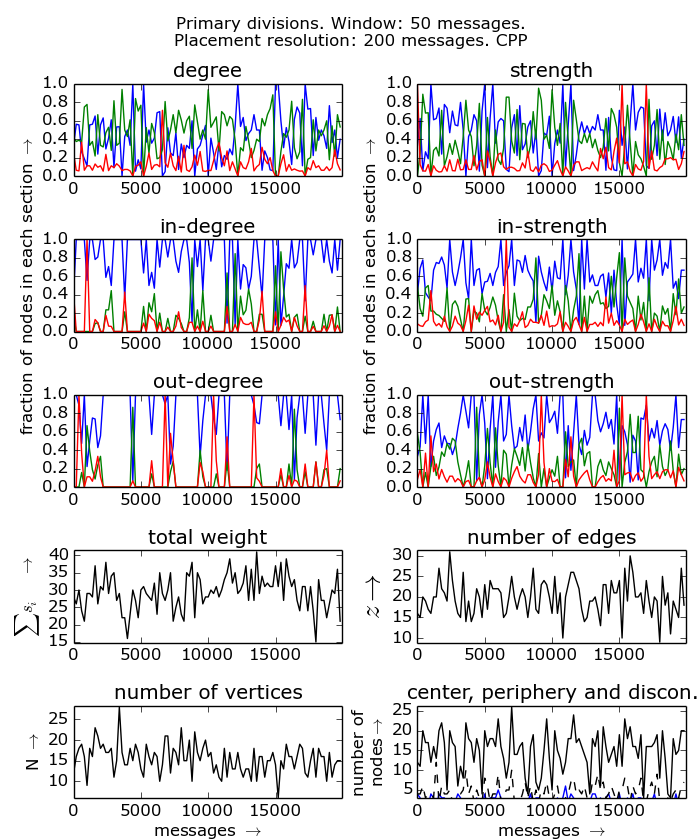
\includegraphics[width=\textwidth]{evoTimelines/evoTimelineCPP-50/CPP-W50-S200}
\end{figure*}
\begin{figure*}
   \centering
        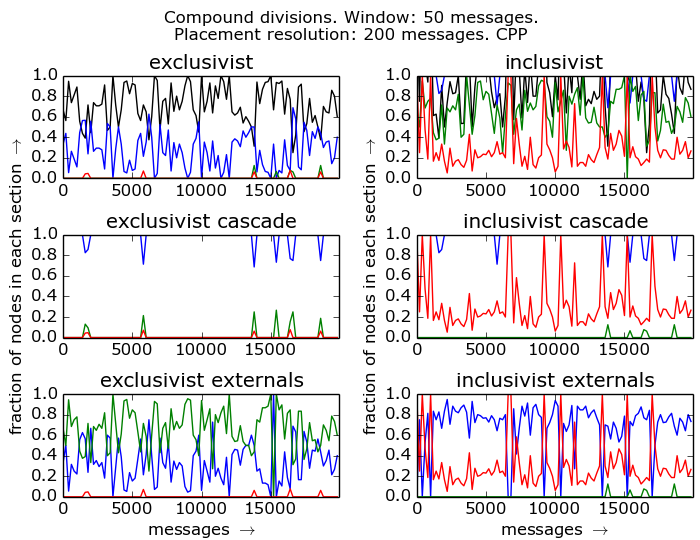
\includegraphics[width=\textwidth]{evoTimelines/evoTimelineCPP-50/CPP-W50-S200_}
\end{figure*}

\begin{figure*}
   \centering
        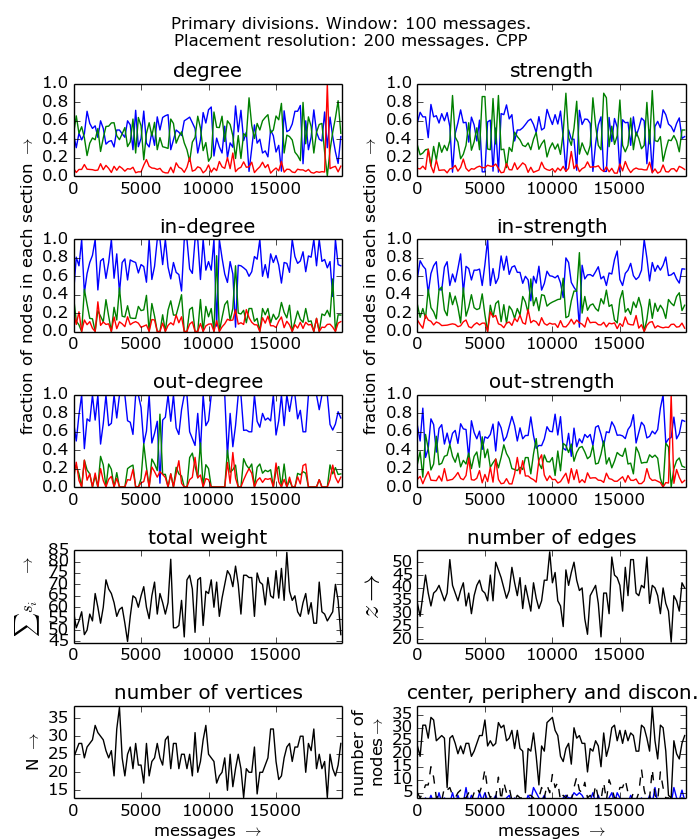
\includegraphics[width=\textwidth]{evoTimelines/evoTimelineCPP-100/CPP-W100-S200}
\end{figure*}
\begin{figure*}
   \centering
        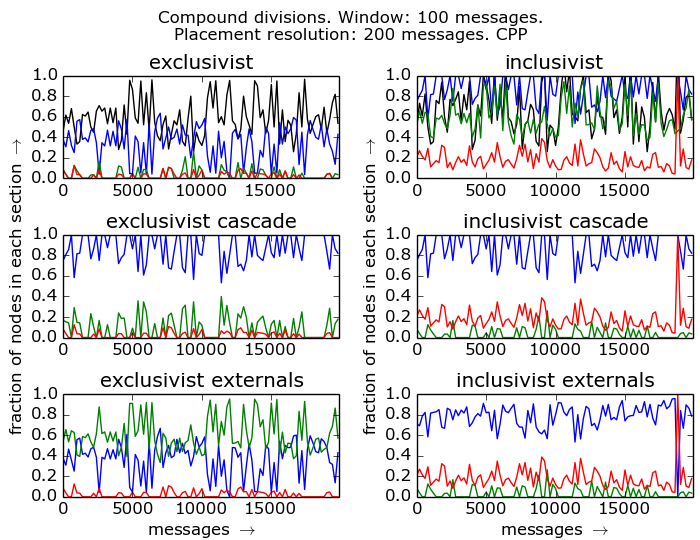
\includegraphics[width=\textwidth]{evoTimelines/evoTimelineCPP-100/CPP-W100-S200_}
\end{figure*}

\begin{figure*}
   \centering
        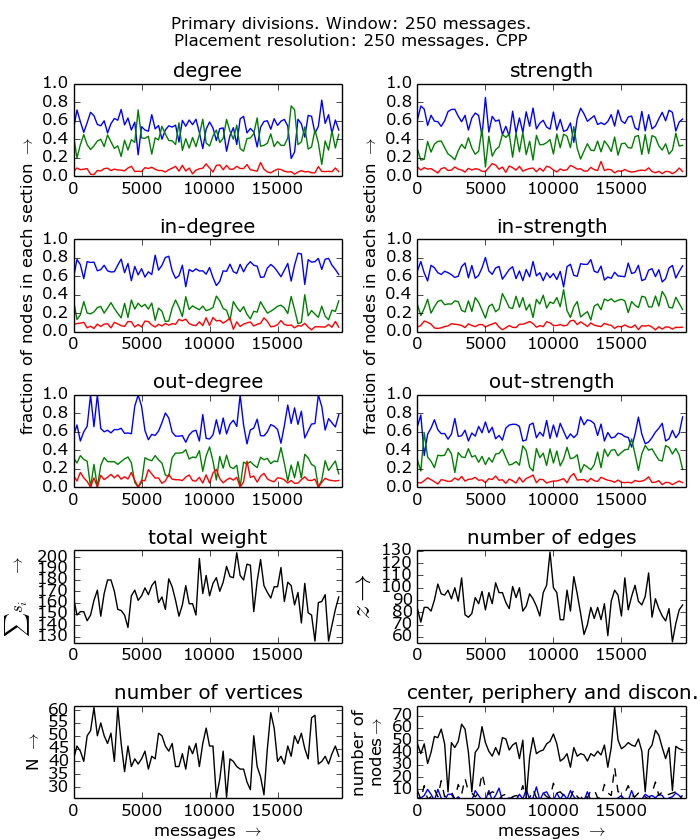
\includegraphics[width=\textwidth]{evoTimelines/evoTimelineCPP-250/CPP-W250-S250}
\end{figure*}
\begin{figure*}
   \centering
        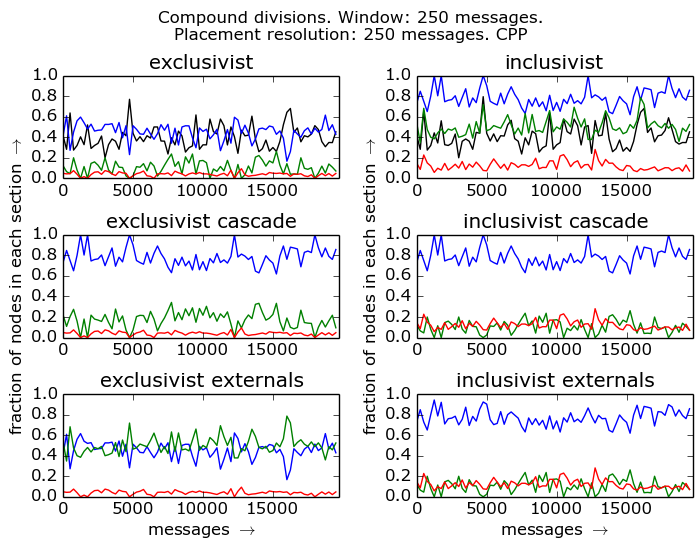
\includegraphics[width=\textwidth]{evoTimelines/evoTimelineCPP-250/CPP-W250-S250_}
\end{figure*}

\begin{figure*}
   \centering
        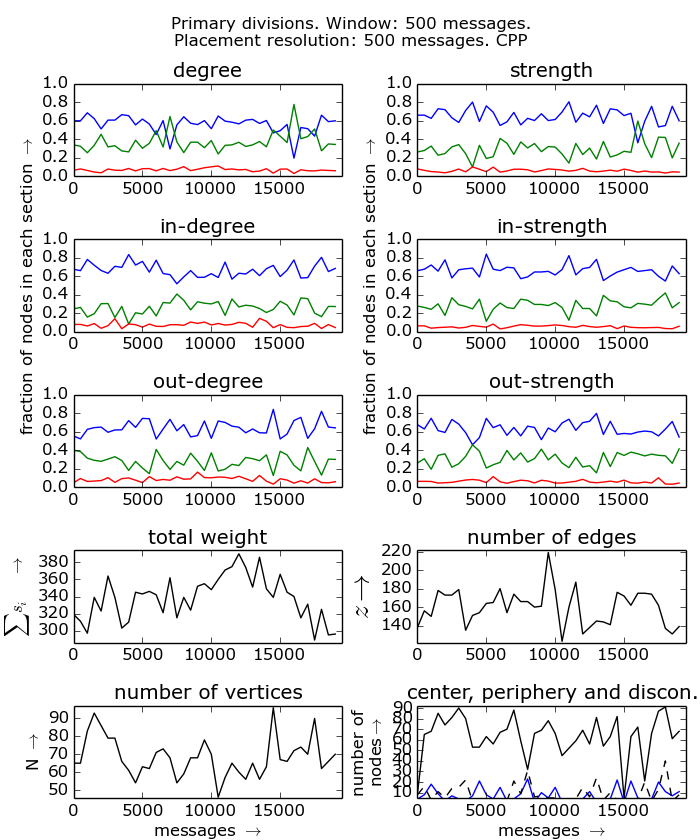
\includegraphics[width=\textwidth]{evoTimelines/evoTimelineCPP-500/CPP-W500-S500}
\end{figure*}
\begin{figure*}
   \centering
        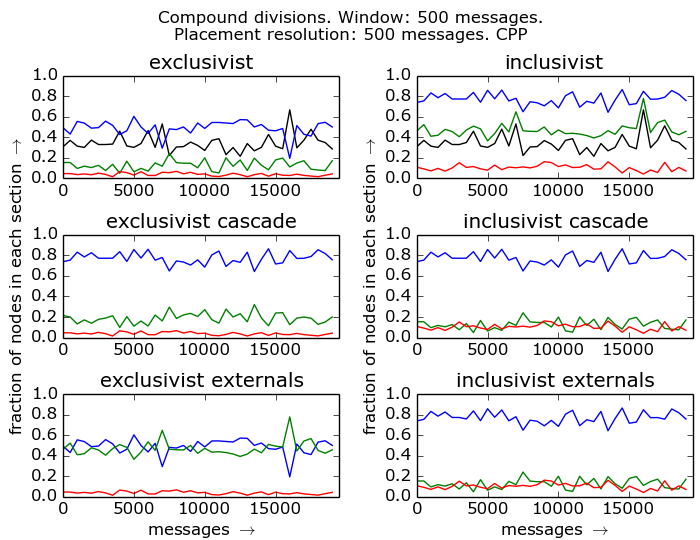
\includegraphics[width=\textwidth]{evoTimelines/evoTimelineCPP-500/CPP-W500-S500_}
\end{figure*}

\begin{figure*}
   \centering
        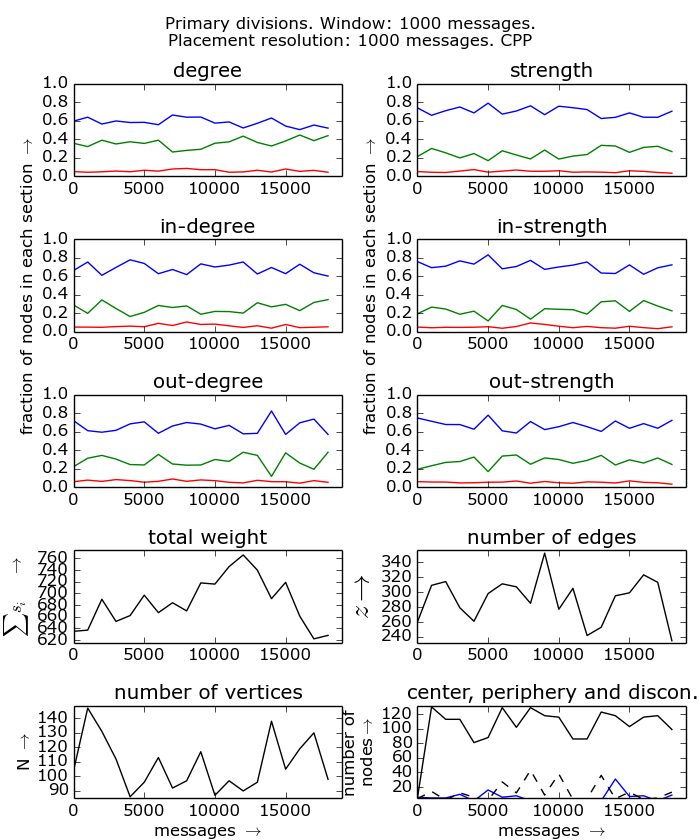
\includegraphics[width=\textwidth]{evoTimelines/evoTimelineCPP-1000/CPP-W1000-S1000}
\end{figure*}
\begin{figure*}
   \centering
        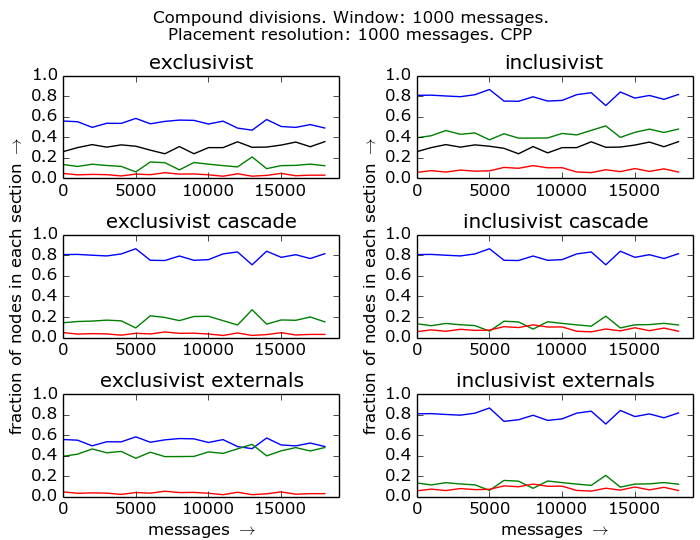
\includegraphics[width=\textwidth]{evoTimelines/evoTimelineCPP-1000/CPP-W1000-S1000_}
\end{figure*}

\begin{figure*}
   \centering
        \includegraphics[width=\textwidth]{evoTimelines/evoTimelineCPP-5000/CPP-W5000-S5000}
\end{figure*}
\begin{figure*}
   \centering
        \includegraphics[width=\textwidth]{evoTimelines/evoTimelineCPP-5000/CPP-W5000-S5000_}
\end{figure*}


\begin{figure*}
   \centering
        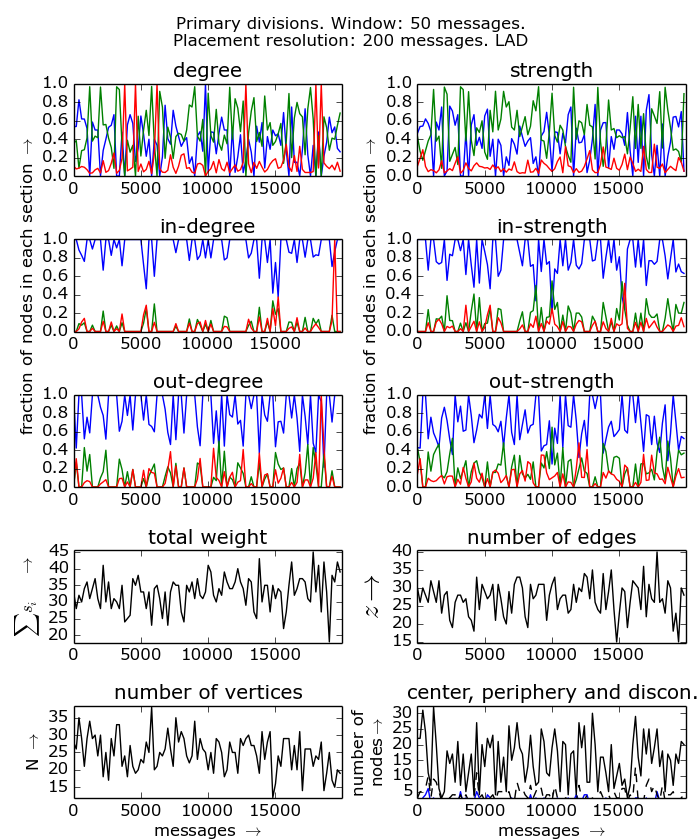
\includegraphics[width=\textwidth]{evoTimelines/evoTimelineLAD-50/LAD-W50-S200}
\end{figure*}
\begin{figure*}
   \centering
        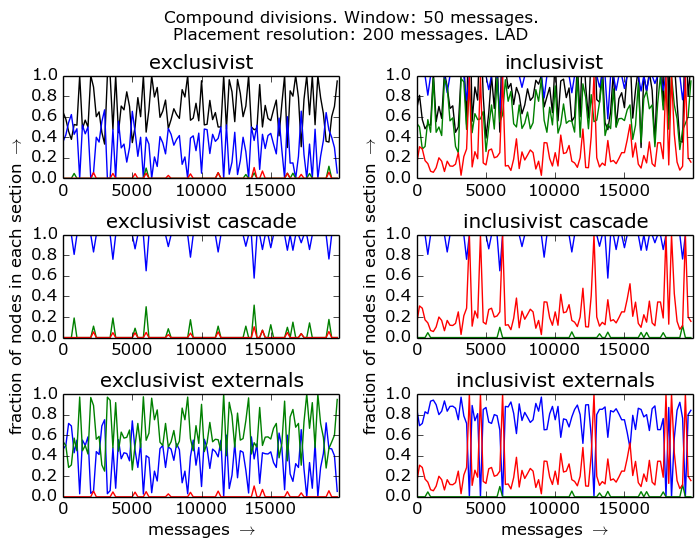
\includegraphics[width=\textwidth]{evoTimelines/evoTimelineLAD-50/LAD-W50-S200_}
\end{figure*}

\begin{figure*}
   \centering
        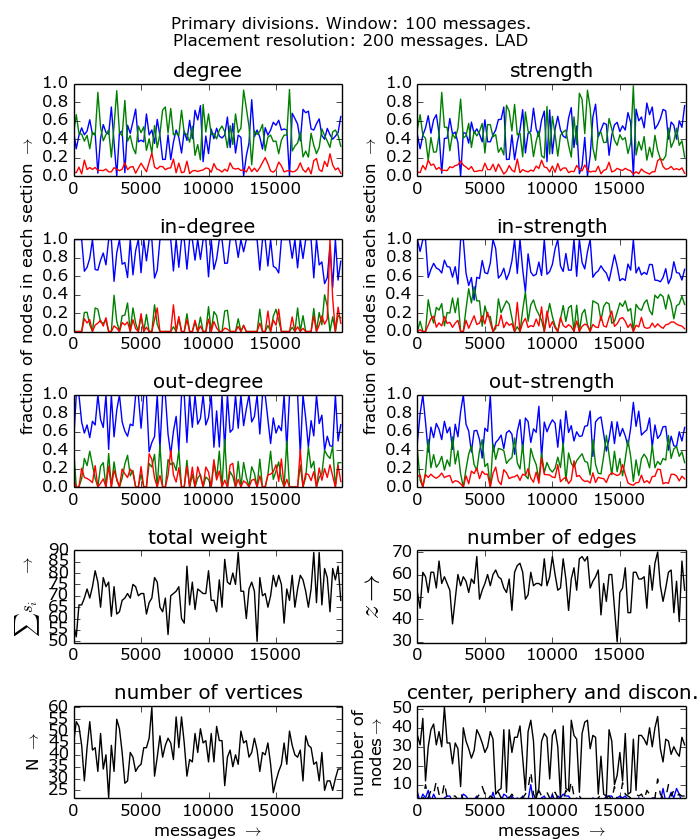
\includegraphics[width=\textwidth]{evoTimelines/evoTimelineLAD-100/LAD-W100-S200}
\end{figure*}
\begin{figure*}
   \centering
        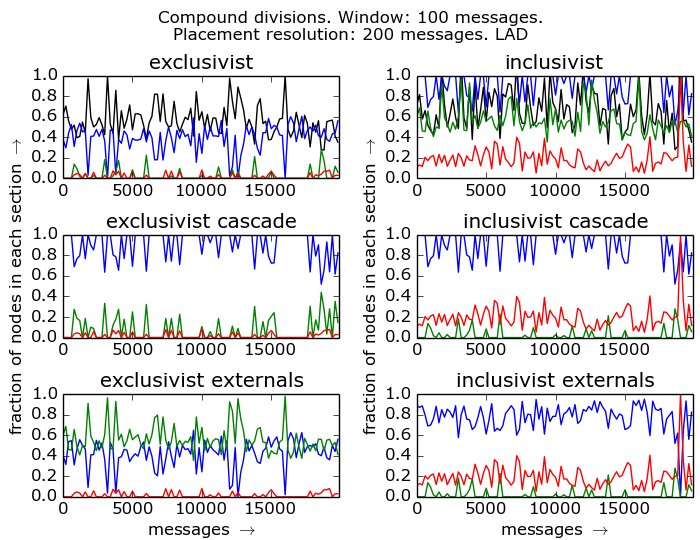
\includegraphics[width=\textwidth]{evoTimelines/evoTimelineLAD-100/LAD-W100-S200_}
\end{figure*}

\begin{figure*}[!h]
   \centering
        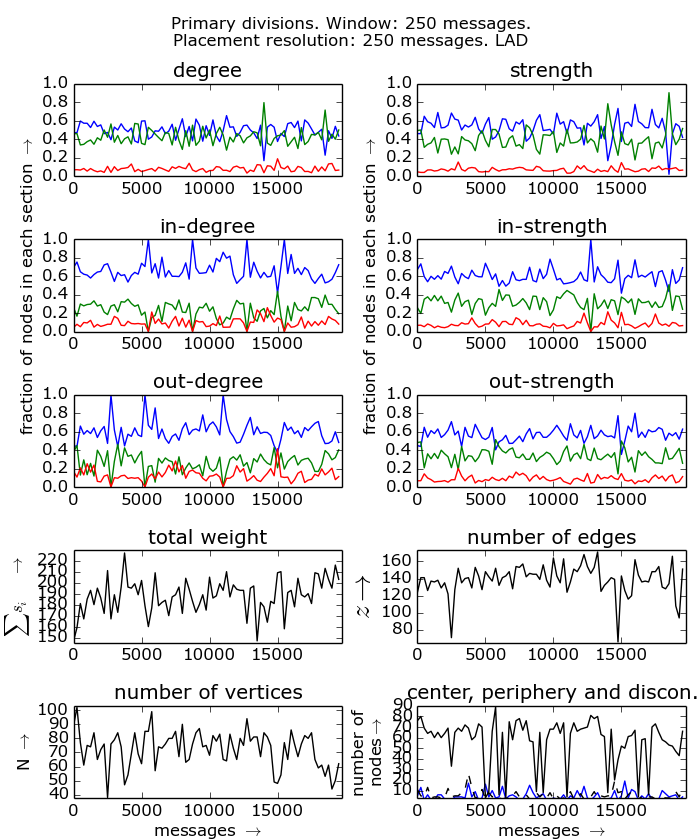
\includegraphics[width=\textwidth]{evoTimelines/evoTimelineLAD-250/LAD-W250-S250}
\end{figure*}
\begin{figure*}
   \centering
        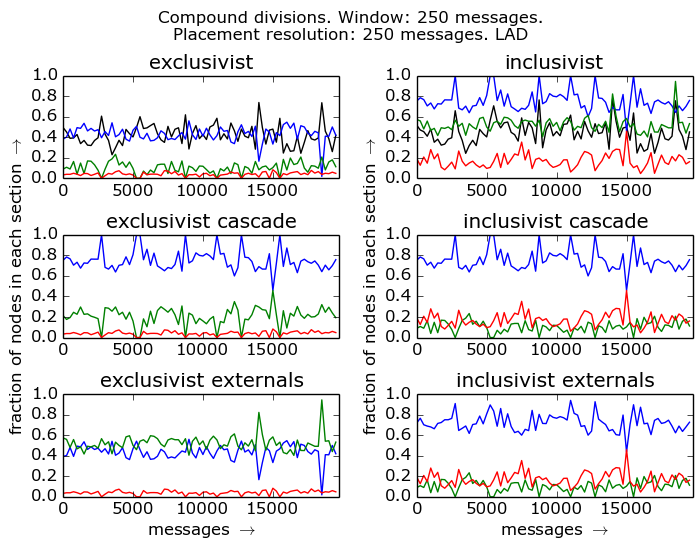
\includegraphics[width=\textwidth]{evoTimelines/evoTimelineLAD-250/LAD-W250-S250_}
\end{figure*}

\begin{figure*}
   \centering
        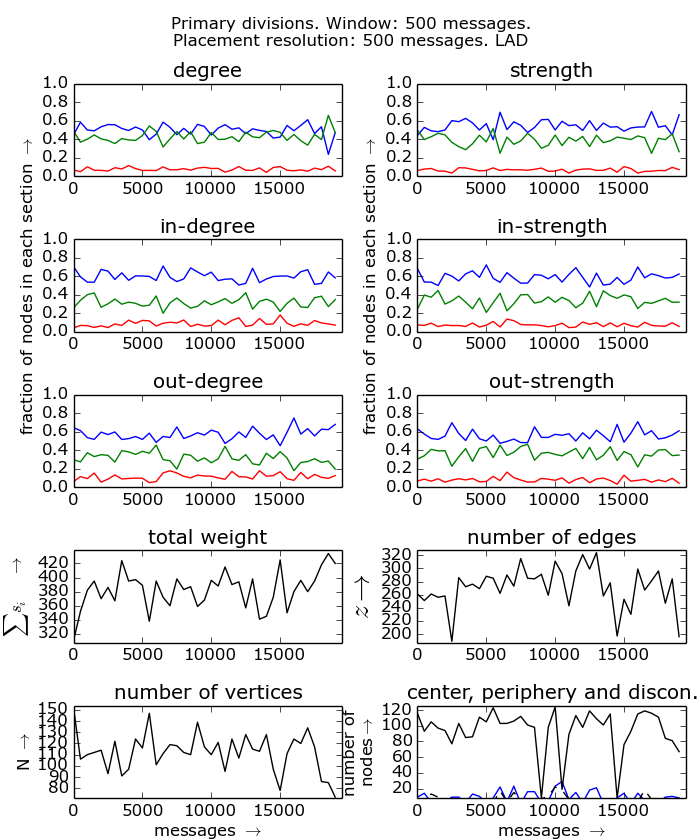
\includegraphics[width=\textwidth]{evoTimelines/evoTimelineLAD-500/LAD-W500-S500}
\end{figure*}
\begin{figure*}
   \centering
        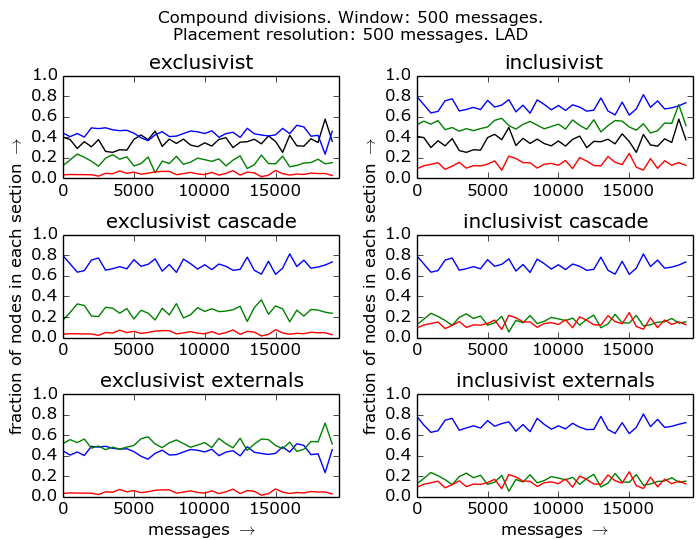
\includegraphics[width=\textwidth]{evoTimelines/evoTimelineLAD-500/LAD-W500-S500_}
\end{figure*}

\begin{figure*}
   \centering
        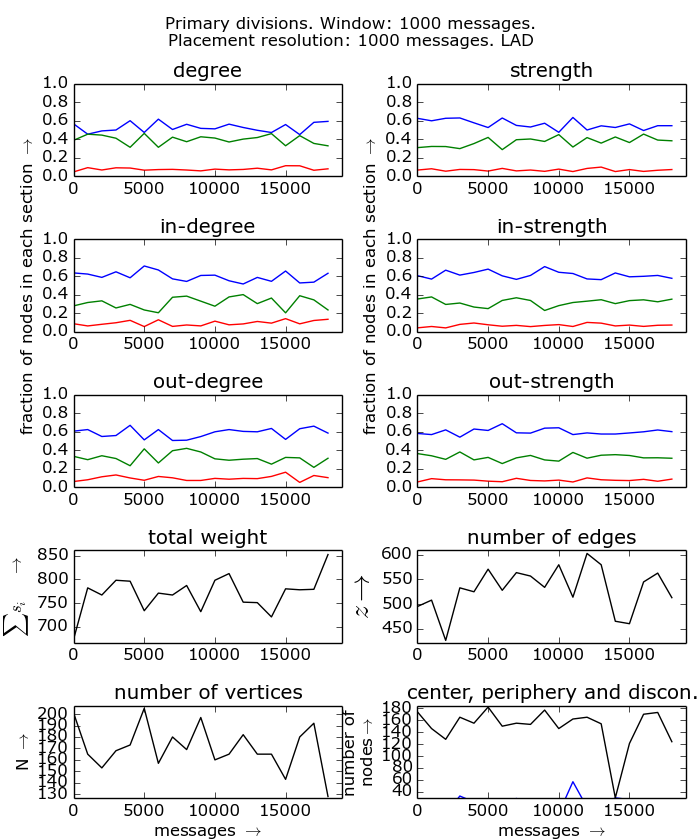
\includegraphics[width=\textwidth]{evoTimelines/evoTimelineLAD-1000/LAD-W1000-S1000}
\end{figure*}
\begin{figure*}
   \centering
        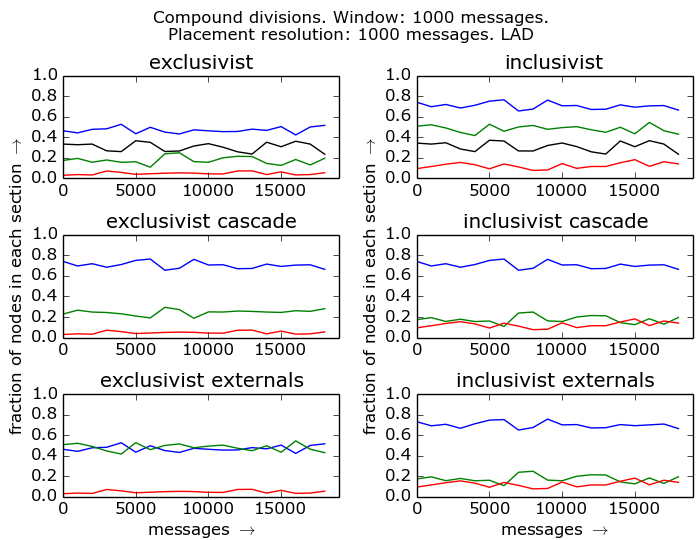
\includegraphics[width=\textwidth]{evoTimelines/evoTimelineLAD-1000/LAD-W1000-S1000_}
\end{figure*}

\begin{figure*}
   \centering
        \includegraphics[width=\textwidth]{evoTimelines/evoTimelineLAD-5000/LAD-W5000-S5000}
\end{figure*}
\begin{figure*}
   \centering
        \includegraphics[width=\textwidth]{evoTimelines/evoTimelineLAD-5000/LAD-W5000-S5000_}
\end{figure*}







\FloatBarrier
\section{PCA of measures along the timeline}\label{sec:pcat}
\subsection{Betweenness, clustering and degree}
\subsection{Betweenness, clustering, degrees and strengths}
\subsection{Betweenness, clustering, degrees, strengths and symmetry measures}

\nocite{*}
\bibliography{supportingInformation}% Produces the bibliography via BibTeX.
\end{document}
%
% ****** End of file aipsamp.tex ******


